% results_v2.tex -- Results section for LLM Overcorrection paper
% All numbers from results_FINAL.md (2026-06-11 corrected/stripped basis).
% Framing: the finding is quality degradation under undirected revision.
% Meta-commentary is a measurement challenge solved in Methods.

\section{Results}
\label{sec:results}

We report meta-commentary-stripped quality scores as our primary estimates throughout; unstripped values are given in parentheses for transparency. Section~\ref{sec:methods-stripping} describes the stripping procedure and its validation.

%% ═══════════════════════════════════════════════════════════════════
%% BLOCK 1: REVISION BEHAVIOR
%% ═══════════════════════════════════════════════════════════════════

\subsection{Models Mostly Decline to Revise}

Offered the balanced probe at each turn, models produce genuine revised content at a declining rate (Table~\ref{tab:revision-rate}). By Turn~5, only 13.3\% of trials contain a genuine revision; the remaining 86.7\% are meta-responses: polite declines, restatements of the original, or commentary about the work rather than new task content.

\begin{table}[t]
    \centering
    \small
    \begin{tabular}{lcc}
    \toprule
    Turn & Genuine revisions & Rate \\
    \midrule
    T2 & 283/720 & 39.3\% \\
    T3 & 185/720 & 25.7\% \\
    T4 & 154/720 & 21.4\% \\
    T5 & 96/720 & 13.3\% \\
    \bottomrule
    \end{tabular}
    \caption{Genuine revision rate by turn. Classifications from a validated LLM classifier (Claude Sonnet~4 at temperature~0; see Section~\ref{sec:methods-classifier}). The majority of post-Turn~1 outputs are meta-responses, not revisions.}
    \label{tab:revision-rate}
\end{table}

\paragraph{Survival varies by model.}
Genuine-revision survival to Turn~5 ranges from 0.8\% (Gemini~2.5 Flash: 1/120 trials) to 53.3\% (Llama~3.3~70B: 64/120). Gemini declines in 98.3\% of post-Turn~1 observations, the most extreme case. Figure~\ref{fig:survival-curves} shows the per-model survival curves; only Llama sustains revision to the final turn. The balanced panel of 50 trials with genuine revision at all turns is composed of 45 Llama trials (90\%), 3 Qwen, and 2 Claude; GPT-4o, DeepSeek, and Gemini contribute zero trials each. This subset conditions on a post-treatment variable (revision persistence), introducing potential selection bias; we triangulate it against the pooled estimates below.

\FloatBarrier
\begin{figure}[!tbp]
    \centering
    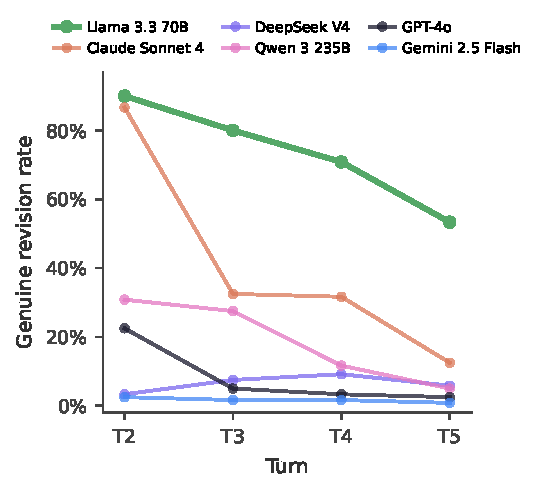
\includegraphics[width=\columnwidth]{figures/fig_survival_curves.pdf}
    \caption{Per-model genuine-revision survival. Fraction of each model's 120 trials still producing genuine revised content at each turn. Llama~3.3~70B sustains revision through Turn~5 (53.3\%); all other models drop below 15\% by Turn~5. Gemini~2.5 Flash is near floor throughout (0.8\% at T5).}
    \label{fig:survival-curves}
\end{figure}
Across five probe wordings the revision gate is bimodal rather than graded; Appendix~\ref{sec:appendix-study1} reports the breakdown. Study~3's balanced probe sits in the assessment range at 39.3\% at Turn~2.


\subsection{Quality Degrades Under Undirected Revision}

% TKTK Liam: statistical plumbing, written to match the surrounding register.
% Every value traces to results_FINAL.md section 4b; script scripts/study3/revision_direction.py.
% Rewrite the prose in your own voice; do not change the numbers without the ledger.
\paragraph{Revisions lower quality more often than they raise it.}
Across all 718 genuine revisions, a revision leaves the quality level unchanged in 62.7\% of
cases, lowers it in 25.6\%, and raises it in 11.7\%. Restricting to the 268 revisions that move
the level at all, 184 move it down and 84 move it up, a share of 68.7\% (exact binomial
95\% CI $[62.8\%, 74.1\%]$; sign test $p = 1.13 \times 10^{-9}$). Of the 524 revisions whose input was already at or above the sufficiency threshold, 144 (27.5\%) end below it. The asymmetry is present in
every model and in every domain, and is significant in four of the six models individually
(Appendix~\ref{sec:secondary-tables}). Unstripped, the same share is 76.6\% (245 against 75,
$p = 1.7 \times 10^{-22}$).

\paragraph{The effect depends on the quality of the input.} In an exploratory analysis that was not among our registered
predictions, the expected change from a single undirected revision varies with the level of
the input being revised
(Figure~\ref{fig:input-level}, Appendix~\ref{sec:supp-figures}): revision raises quality when the input falls below the
sufficiency threshold ($+0.41$, $n = 194$) and lowers it when the input is already
sufficient ($-0.56$, $n = 524$).

\paragraph{The revision cliff.}
In the 50 balanced-panel trials (genuine revision at all turns), the two ways an output can
fail move in opposite directions. Nineteen trials became over-elaborated by Turn~5 and one
moved the other way (exact binomial $p = 4.01 \times 10^{-5}$), taking the share rated
``Overdone'' from 4\% to 40\%, while the share falling below sufficiency does not change (5
in, 11 out, $p = 0.21$). Undirected revision adds unrequested material; it does not drop what
was asked for. On the ordinal scale, mean quality on stripped content falls from 3.70 to 3.32,
a decline of $-0.38$ levels ($p = 4.42 \times 10^{-3}$; unstripped $-0.44$, $p = 3.8 \times
10^{-4}$), of which 14\% is attributable to meta-commentary rather than to content.
``Overdone'' is placed at level~3 throughout, since an over-elaborated output contains every
requested component: the fault is the kind of weakness level~3 names, not the absence level~2
names. The count above does not depend on that placement.
The balanced panel is dominated by Llama~3.3~70B ($n = 45$), the only model with power
to detect a within-model cliff; its stripped cliff of $-0.31$ is significant at $p = 1.80 \times 10^{-2}$. GPT-4o, DeepSeek and Gemini contribute no balanced-panel trials,
not because they hold quality but because they stop revising before Turn~5. We do not claim
all models degrade; we claim that among models that continue revising, the only powered
comparison shows significant degradation.

\paragraph{Pooled trajectory.} Pooling all genuine revisions with shifting $n$, stripped
quality falls from 4.17 at Turn~1 to 3.42 at Turn~5 ($\Delta = -0.75$). This estimator uses
every genuine revision rather than the balanced panel, but introduces a compositional bias:
models with higher decline rates exit the pool earlier. The direction agrees with the
balanced-panel estimate, and Figure~\ref{fig:quality-trajectory} plots both.

\FloatBarrier
\begin{figure}[!tbp]
    \centering
    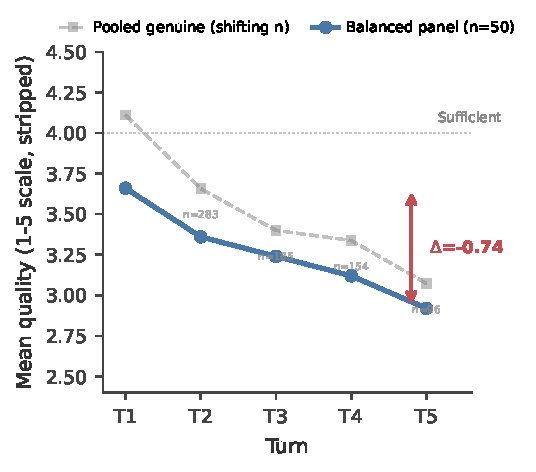
\includegraphics[width=\columnwidth]{figures/fig_quality_trajectory.pdf}
    \caption{Quality trajectory under undirected revision (stripped scores). Solid blue: balanced panel ($n = 50$, genuine revision at all turns), showing the balanced-panel cliff of $\Delta = -0.38$ (3.70$\to$3.32). Dashed gray: pooled genuine-only trajectory, $\Delta = -0.75$; its $n$ falls from 283 at Turn~2 to 96 at Turn~5 as models stop revising, which is the compositional bias that estimator carries. Both estimators decline monotonically. The dashed horizontal line marks the sufficiency threshold (level~4).}
    \label{fig:quality-trajectory}
\end{figure}
With probe phrasing held constant, model identity explains far more variation in
genuine-revision rate than task domain: a range of 71.9 percentage points against 13.5. All
five domains show negative stripped deltas, three of five significant on paired Wilcoxon tests;
per-domain Turn~5 cells run from $n = 13$ to $n = 30$, so these are directional
(Appendix~\ref{sec:secondary-tables}).

\paragraph{Revision despite sufficiency.}
The evaluator rated 87.6\% of first-turn outputs as sufficient (631/720), so most trials begin
with work that needs no revision. Among all (trial, turn) pairs where the output was rated
sufficient (level $\geq 4$), the model produced a genuine revision at the next turn 39.6\% of the time (411/1,038 sufficient turns; unstripped 39.2\%).

%% ═══════════════════════════════════════════════════════════════════
%% BLOCK 3: TARGETED FEEDBACK
%% ═══════════════════════════════════════════════════════════════════

% TKTK: assembled 2026-09-16 from the sentence that was in limitations.tex and the
% numbers in methods.tex, so no figure here is new. Voice pass yours. Placed after the
% degradation finding because it qualifies that finding directly; move it if you would
% rather the section keep closing on the revision tax.
\subsection{Readers Cannot Reliably Tell the Drafts Apart}
\label{sec:reversibility}

Two annotators compared stripped first drafts against stripped final revisions. Turn~1
was preferred in 41 of 73 decided
comparisons (56.2\%, bootstrap 95\% CI [45.2\%, 67.1\%]; 27 of the 100 pooled judgments
were ties, $\kappa = 0.703$). We set a bar in advance of $\geq$65\% Turn~1 preference with
a confidence interval excluding 50\%. That bar was not cleared, and the interval includes
chance, so we do not claim a reader can reliably pick the first draft.
This bounds what the degradation means in practice without touching what it measures. The
drop of 0.38 levels is not large enough to reverse a blind pairwise preference once
meta-commentary is removed, and its form explains why: an over-elaborated draft reads as more
polished than the one it replaced. What declines is measured quality against the stated task,
not the impression the text leaves.

\subsection{Targeted Feedback Raises Quality on Insufficient Work}
\label{sec:targeted}

Where the evaluator rated an output below the sufficiency threshold, a second instance received that output plus a written critique and produced what we call a targeted revision. On stripped content, targeted revisions score 4.71 against 3.70 for the model's own generic next-turn revision, a gain of 1.01 levels ($p = 1.9 \times 10^{-19}$, $n = 177$; unstripped: 4.71 against 4.51, $+0.20$, $p = 6.6 \times 10^{-3}$). The unstripped comparison understates the real effect because meta-commentary on generic revisions inflates their scores; targeted revisions contain minimal meta-commentary (9/177 = 5\%).
This effect is significant for all five models with sufficient sample size (Table~\ref{tab:targeted-per-model}); on unstripped text only Claude and DeepSeek reach significance, the other generic baselines being inflated by meta-commentary.

\begin{table}[t]
    \centering
    \small
    \begin{tabular}{lccc}
    \toprule
    Model & $n$ & Stripped $\Delta$ & $p$ \\
    \midrule
    Llama 3.3 70B & 71 & $+1.62$ & $9.2 \times 10^{-12}$ \\
    Qwen 3 235B & 21 & $+1.48$ & $4.5 \times 10^{-4}$ \\
    GPT-4o & 12 & $+1.33$ & $7.8 \times 10^{-3}$ \\
    DeepSeek V4 Flash & 19 & $+1.05$ & $1.5 \times 10^{-2}$ \\
    Claude Sonnet 4 & 51 & $+0.31$ & $1.2 \times 10^{-2}$ \\
    Gemini 2.5 Flash & 3 & $+2.33$ & -- ($n < 5$) \\
    \bottomrule
    \end{tabular}
    \caption{Targeted-feedback advantage by model on stripped content, over pairs whose input was rated below sufficiency. All five powered models show significant improvement.}
    \label{tab:targeted-per-model}
\end{table}

Undirected revision costs 0.38 levels across the balanced panel, 33 of whose 50 trials begin above the sufficiency threshold. A critique naming the fault raises quality by 1.01 levels on work rated below it.

\FloatBarrier

%% ═══════════════════════════════════════════════════════════════════
%% BLOCK 4: REVISION TAX
%% ═══════════════════════════════════════════════════════════════════

\subsection{The Revision Tax}

The quality-optimal stopping point ($t^*$) is Turn~1 for all six models: no model benefits from undirected revision on the genuine-revision quality trajectory. All tokens generated after Turn~1 are therefore waste under a quality-maximizing criterion. There are two views of the same waste. As a share of all output, 62.1\% of tokens across the
720 trials are spent past $t^*$ (Figure~\ref{fig:revision-tax}); measured against only the
tokens needed to reach $t^*$, the waste is 164.2\%, so continuing past peak quality produces
roughly 1.6 times more text than reaching the optimum took. Per-model waste ranges from 23.4\% (Gemini, which declines early and generates few post-T1 tokens) to 81.3\% (Llama, which continues revising and generates substantial post-T1 content). 

\subsection{Scoring Restraint}
\label{sec:stet}

The forty tasks, the five-turn protocol and the scoring procedure define a diagnostic we
call STET, after the editor's mark that lets text stand. It scores one behaviour: the share
of already-sufficient output a model leaves alone (Table~\ref{tab:stet}).

\begin{table}[t]
\centering
\small
\begin{tabular}{@{}lr@{}}
\toprule
Model & Sufficient output left alone \\
\midrule
Gemini 2.5 Flash & 97.8\% \\
DeepSeek V4 Flash & 96.3\% \\
GPT-4o & 82.3\% \\
Qwen 3 235B & 68.4\% \\
Claude Sonnet 4 & 54.1\% \\
Llama 3.3 70B & 18.4\% \\
\bottomrule
\end{tabular}
\caption{Share of turns rated sufficient whose next turn is not a genuine revision,
stripped basis, over 36 of the 40 tasks; four Gemini cells contain no sufficient turn and
so no denominator.}
\label{tab:stet}
\end{table}

Whether forty tasks rank six models stably is testable. Across 1,000 random splits of the tasks into halves, the halves agree at mean Spearman $\rho = 0.972$,
every split clears $0.80$, and Llama is last in all of them. A generalizability decomposition gives $G = 0.992$ over the 36 tasks that carry a denominator, where six would reach $0.95$, because variance between models is 3.2 times the model-by-task residual. Genuine-revision rate and
the revision tax order the models identically ($\rho = 1.000$), so we report one of the three.

The decline itself is not scoreable this way, and we do not score it. No construction of the Turn~1 to Turn~5 delta holds its \emph{ordering of models} across task halves in more than 11\% of draws, and its $G$ of 0.780 would need 215 tasks: across the six models that delta correlates $-1.000$ with mean Turn~1 quality, so it separates models by where they start rather than by how far they fall. This bears on using the decline as a per-model score, not on its magnitude.

\begin{figure}[t]
    \centering
    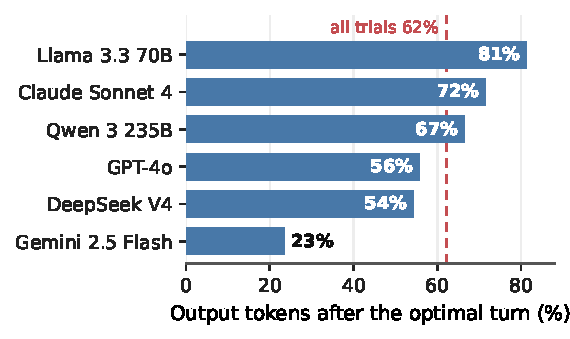
\includegraphics[width=\columnwidth]{figures/fig_revision_tax.pdf}
    \caption{Share of each model's output tokens generated after the quality-optimal stopping point,
    which is Turn~1 for all six. Meta-response tokens count as waste. The dashed line is
    the all-trials aggregate.}
    \label{fig:revision-tax}
\end{figure}

% ═══════════════════════════════════════════════════════════════════
% FLAGS: Spec-data misalignments
% ═══════════════════════════════════════════════════════════════════
%
% FLAG 1 [RESOLVED 2026-07-23]: The 98.3% Gemini decline rate is now VERIFIED by
%   direct computation from genuine_meta_labels.jsonl: Gemini META = 472/480
%   post-Turn-1 observations = 98.3% (exact). Per-model META rates: Gemini 98.3%,
%   DeepSeek 93.5%, GPT-4o 91.7%, Qwen 81.2%, Claude 59.2%, Llama 26.5%.
%
% FLAG 2: The stripped balanced-panel cliff uses -0.38 from the full
%   3,600-output rescore, with Overdone placed at level 3 per
%   scripts/config.OVERDONE_RANK. It was -0.74 when Overdone was placed
%   at level 2; see results_FINAL.md sections 19, 19b and 20 for the four
%   codings, the human-rater evidence and the decision.
